\section{pcan\-\_\-receive.\-cpp \-File \-Reference}
\label{pcan__receive_8cpp}\index{pcan\-\_\-receive.\-cpp@{pcan\-\_\-receive.\-cpp}}
{\ttfamily \#include $<$stdio.\-h$>$}\*
{\ttfamily \#include $<$stdlib.\-h$>$}\*
{\ttfamily \#include $<$errno.\-h$>$}\*
{\ttfamily \#include $<$unistd.\-h$>$}\*
{\ttfamily \#include $<$signal.\-h$>$}\*
{\ttfamily \#include $<$string.\-h$>$}\*
{\ttfamily \#include $<$fcntl.\-h$>$}\*
{\ttfamily \#include $<$libpcan.\-h$>$}\*
{\ttfamily \#include \char`\"{}common.\-h\char`\"{}}\*
{\ttfamily \#include $<$ctype.\-h$>$}\*
{\ttfamily \#include \char`\"{}ros/ros.\-h\char`\"{}}\*
{\ttfamily \#include \char`\"{}std\-\_\-msgs/\-String.\-h\char`\"{}}\*
{\ttfamily \#include $<$sstream$>$}\*
{\ttfamily \#include \char`\"{}pcan\-\_\-receive.\-h\char`\"{}}\*
\-Include dependency graph for pcan\-\_\-receive.\-cpp\-:\nopagebreak
\begin{figure}[H]
\begin{center}
\leavevmode
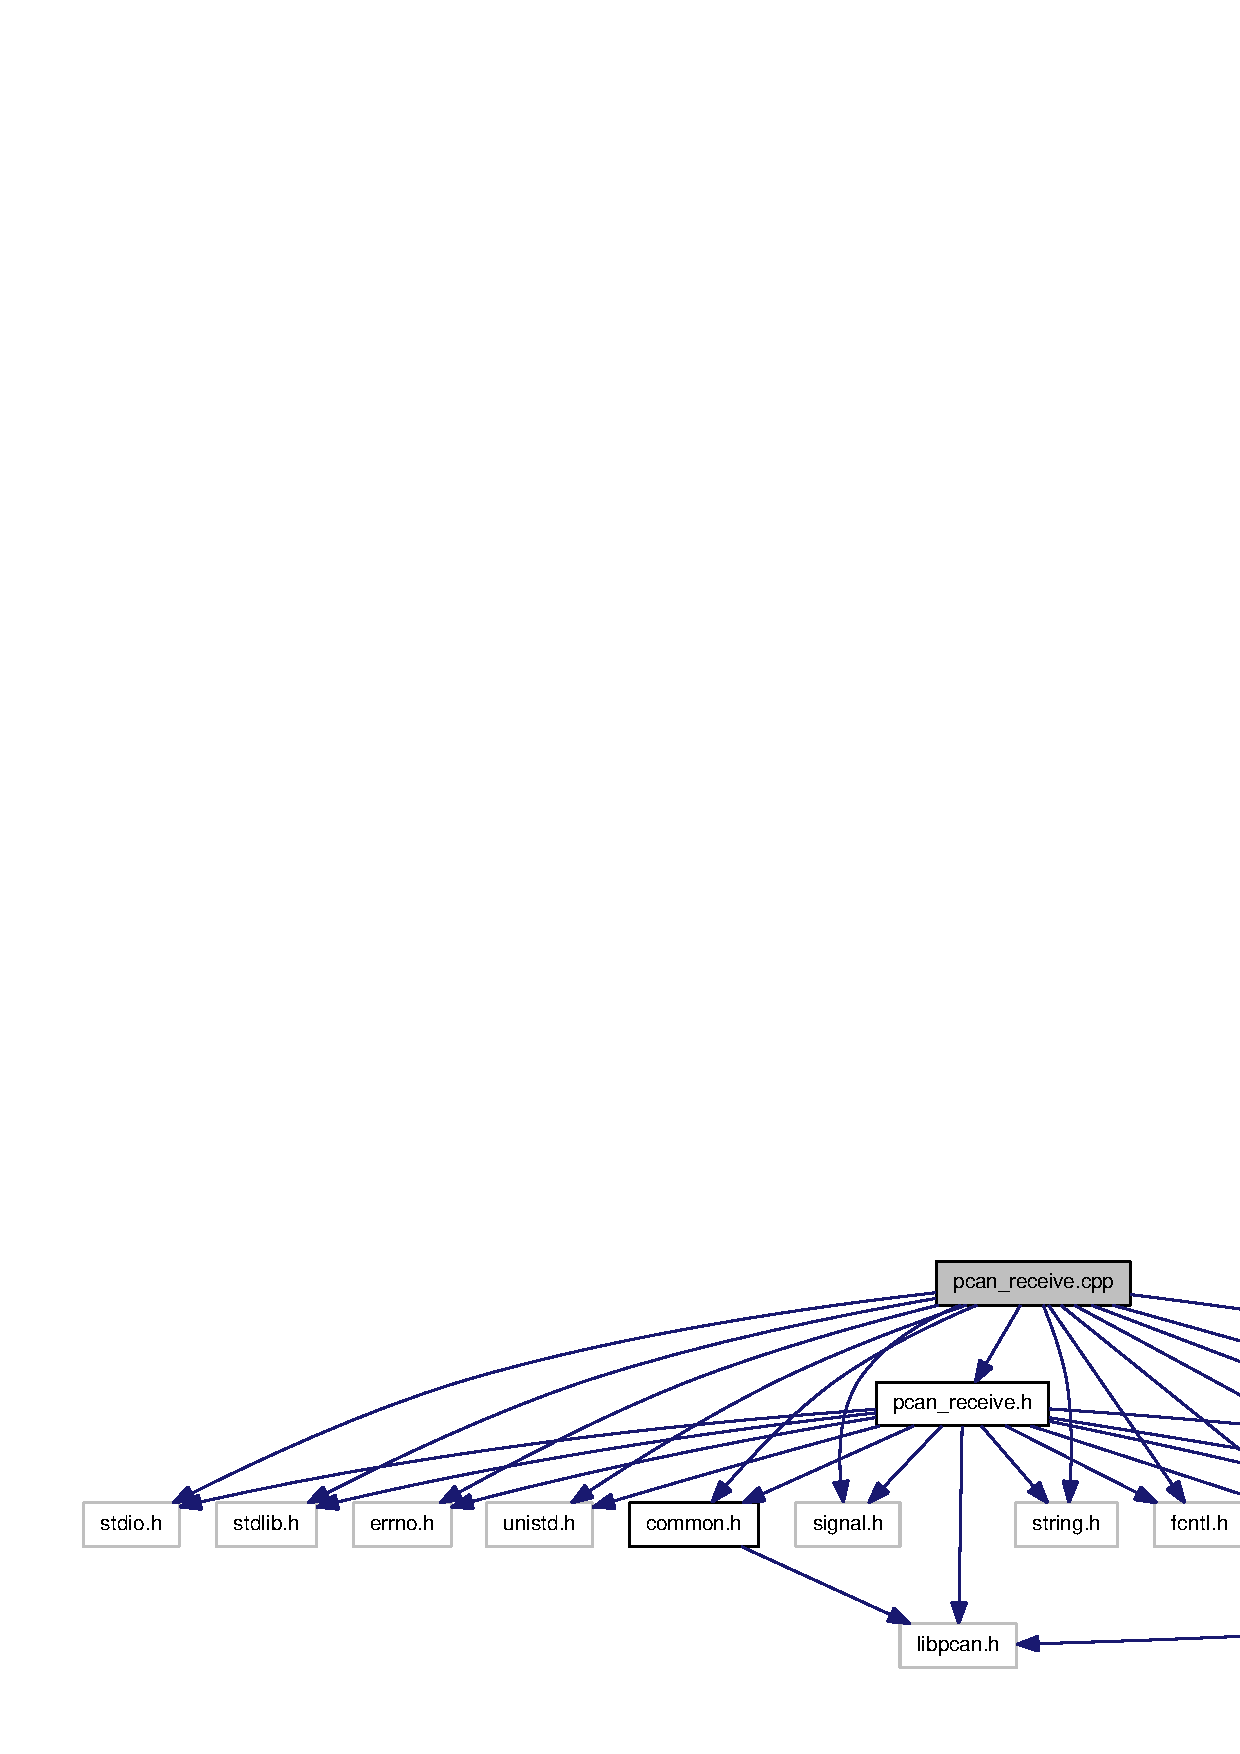
\includegraphics[width=350pt]{pcan__receive_8cpp__incl}
\end{center}
\end{figure}
